\section{Conjecture dans un cas particulier de la capacité unitaire}

\subsection{Modèle et hypothèses}

\begin{frame}[label=CapaciteUnitaire]
  \frametitle{Modèle et hypothèse}
  
  \begin{center}
  
    \begin{minipage}[c]{.5\linewidth}
      \begin{center}
        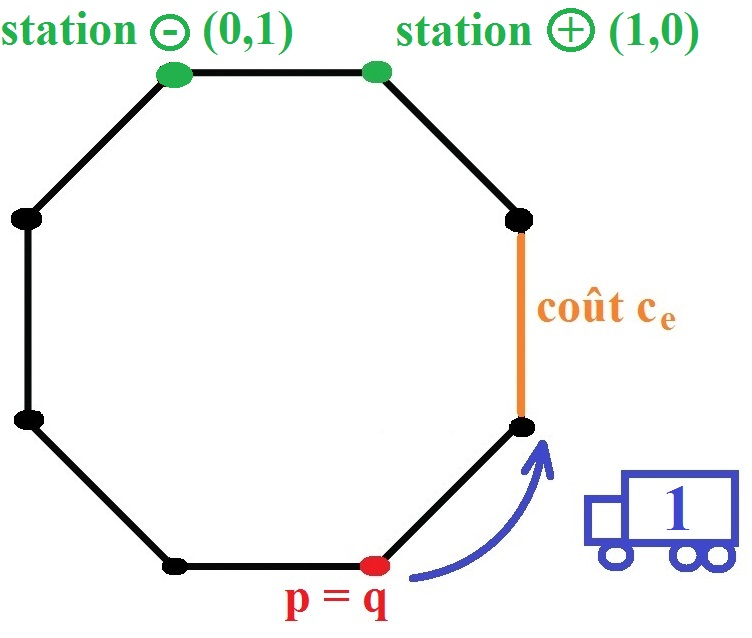
\includegraphics[width=\textwidth]{CapaciteUnitaire/modele.jpg}
      \end{center}
    \end{minipage}\hfill
    \begin{minipage}[c]{.5\linewidth}
      \textbf{Hypothèses (H) :}
      \begin{itemize}
      \item Capacité de transport $C=1$
      \item deux formes de stations possibles :
        \begin{itemize}
        \item station \plus de la forme $(1,0)$
        \item station \moins de la forme $(0,1)$
        \end{itemize}
      \end{itemize}
    \end{minipage}
  \end{center}
  \vfill
  \textbf{Conséquence :} $2n$ stations ($n$ \plus et $n$ \moins)
\end{frame}

\subsection{Conjecture et algorithme polynomial}

\begin{frame}
\frametitle{Conjecture et algorithme polynomial}

\onslide<1->
{
  \begin{conj} \label{conj: capacité unitaire - un passage}
  Sous les hypothèses (H), il existe un trajet optimal et une arête $e_0$ tels que le camion passe au plus une fois par $e_0$ au cours de ce trajet.
  \end{conj}
}
\onslide<2->
{
  \begin{thm} \label{thm: capacité unitaire - optimalité}
  Sous les hypothèses (H) et en supposant la conjecture précédente vraie, il existe un algorithme polynomial donnant le trajet optimal du camion.
  \end{thm}
}
\end{frame}

\begin{frame}
\frametitle{Idées clés de la démonstration}

\begin{proof}
  \begin{itemize}
  \item<1-> il existe $e_0 \in E$ tel que le camion ne passe pas par $e_0$
  \item<2-> le camion passe par tous les sommets et\\
    il existe $e_0 \in E$ tel que le camion passe exactement une fois par $e_0$
    \begin{itemize}
    \item<3-> Construire le graphe biparti complet (\plus et \moins)
    \item<4-> Recherche de cycle hamiltonien optimal $\Rightarrow$ indépendant origine
    \item<5-> On résout à partir de la station atteinte après le passage sur $e_0$\\
    (algorithme dans le cas linéaire)
    \end{itemize}
  \end{itemize}
  \vskip-1\baselineskip
\end{proof}
\onslide<5->
{
  \begin{center}
    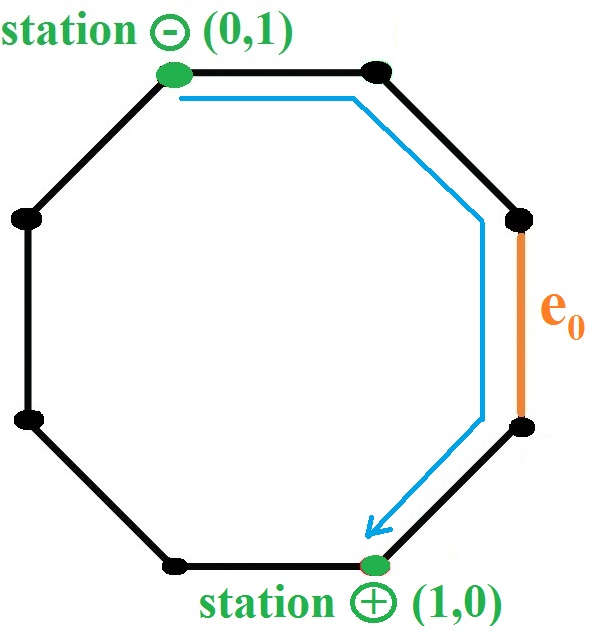
\includegraphics[width=0.35\textheight]{CapaciteUnitaire/PreuveAlgo1.jpg}
    \hspace{2cm}
    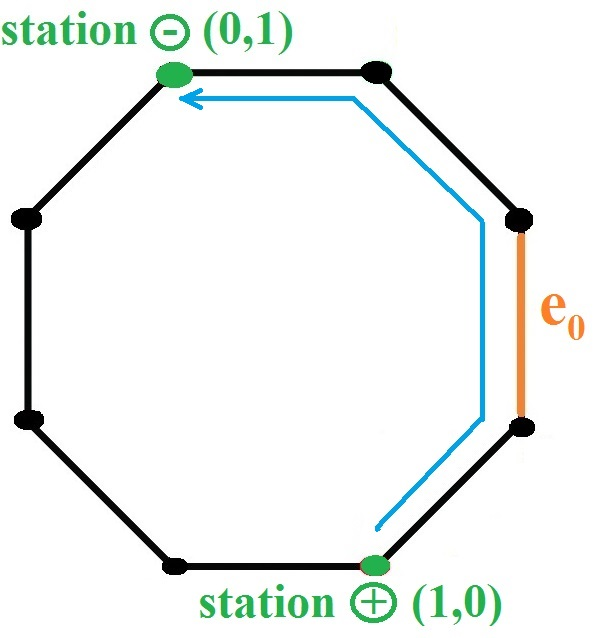
\includegraphics[width=0.35\textheight]{CapaciteUnitaire/PreuveAlgo2.jpg}
  \end{center}
}

\end{frame}


\subsection{Majoration du coût et polynomialité}

\begin{frame}
\frametitle{Majoration du coût et polynomialité}
\onslide<1->
{
  \begin{prop}
  Sous les hypothèses (H), si  $\Upsilon_G$ < $2\sum_{e \in E}c_e$, alors il existe un algorithme polynomial donnant le trajet optimal du camion.
  \end{prop}
}
\onslide<2->
{
  \begin{proof}
  Par l'absurde, si $S$ passe au moins deux fois par chaque arête
  
  alors $\Upsilon_G~\ge~2\sum_{e \in E}c_e$
    \vskip-0.8\baselineskip
  \end{proof}
}

\end{frame}